\documentclass{article}
\usepackage{ctex}
\usepackage[top=3cm,left=2cm,right=2cm,bottom=2cm]{geometry}
\title{治未病问卷小样}
\author{}
\date{}
\usepackage{setspace}
\usepackage{fancyhdr}
\usepackage{graphicx}
\graphicspath{{images/}}
\usepackage{subfigure}
\pagestyle{empty}
\begin{document}
\maketitle
\clearpage

您好,这是一份由南京中医药大学第一临床医学院发起的调查问卷,旨在了解社区居民对于中医治未病理论的认知、行为等情况,响应“健康中国”工程,为后面中医治未病理论的传播做一个描述性统计分析。

本问卷时长约五到十分钟,我们郑重承诺,本问卷的所有数据仅用于科研用途,您的所有个人信息将受到相关法律的保护。

\begin{spacing}{0.9}
\begin{enumerate}
%知识部分
\item 中医学特点之一是整体观,认为“天人合一”,即人的健康受到周围环境(自然、社会、家庭)的影响。您认为:

A.正确\qquad B.部分正确\qquad C.错误 \qquad D.不清楚

\item 中医学认为人应该调节身体状况以适应气候、环境的变化。您认为:

A.正确\qquad B.部分正确\qquad C.错误 \qquad D.不清楚

\item 人的身体是一个整体,一个系统或器官的疾病可以影响其它系统或器官。您认为:

A.正确\qquad B.部分正确\qquad C.错误 \qquad D.不清楚

\item 人的情绪、精神状态对疾病有影响。您认为:

A.正确\qquad B.部分正确\qquad C.错误 \qquad D.不清楚

\item 人的健康与饮食有很大关系,中医的食疗指通过饮食调理来改变人的健康状况。
您认为:

A.正确\qquad B.部分正确\qquad C.错误 \qquad D.不清楚

\item 食物有寒凉等不同属性,人的体质也有阴阳等差别,所以饮食要根据体质不同进行选择。这个观点您认为:

A.正确\qquad B.部分正确\qquad C.错误 \qquad D.不清楚


\item 刮痧、拔火罐、推拿等方法是治未病理论的运用,可以起到增强体质、保护健康的作用。这个说法您认为:

A.正确\qquad B.部分正确\qquad C.错误 \qquad D.不清楚

\item 
治未病是中医特有的理论和方法,西医没有这样的说法,您认为,

A.正确\qquad B.部分正确\qquad C.错误 \qquad D.不清楚

\item 您了解中医养生知识的途径是以下哪些?(可多选)

A.社区宣传\qquad B.亲戚朋友推荐\qquad C.医生\qquad
D.电视\qquad
E.互联网\qquad
F.其他途径(填写)\underline{\makebox[6em]{}}

\item 您认为“治未病”一词的含义是指什么?(可多选)

A.预防未发生的疾病\qquad B.生病后防止病情进展\qquad C.病后预防疾病再次复发

%信念部分
\item 
您相信中医理论有其科学性,能从和西医不同的角度解释和解决疾病问题吗?

A.相信\qquad B.部分相信\qquad C.不相信\qquad D.不好说

\item 您本人能接受中医对您的诊断吗?

A.相信\qquad B.部分相信\qquad C.不相信\qquad D.不好说

\item 中医药的治疗(包括针灸、推拿、中药、中成药)只要选择得当,对治疗大多数疾病有效果,您相信吗?

A.相信\qquad B.部分相信\qquad C.不相信\qquad D.不好说

\item 您本人愿意接受中医药治疗方法吗?

A.愿意\qquad B.部分愿意\qquad C.不愿意 \qquad D.不好说

\item 您本人愿意尝试治未病提供的运动保健(太极拳、气功等)的方法吗?

A.愿意\qquad B.部分愿意\qquad C.不愿意 \qquad D.不好说

\item 您会用中医有关调畅情志的理论和方法来解决心理、情绪上的问题吗?

A.愿意\qquad B.部分愿意\qquad C.不愿意 \qquad D.不好说

\item 您愿意学习中医饮食调理的理论和方法并在日常饮食中加以运用吗?

A.愿意\qquad B.部分愿意\qquad C.不愿意 \qquad D.不好说

\item 您喜欢看养生方面的书籍、视频等资料吗?

A.喜欢\qquad B.一般\qquad C.不喜欢\qquad D.我不清楚


%行为题目
\item
过去一年您接受中医治疗的次数?

A.0次 \qquad
B.1-2次\qquad
C.2-5次\qquad
D.5次以上

\item
您接受了哪一种中医治疗呢?

A.草药煎汤\qquad B.贴敷的膏药\qquad C.物理疗法,比如针灸,拔火罐等\qquad D.填写\underline{\makebox[6em]{}}

\item 您过去服用过几次膏方(固元膏、阿胶膏等等)吗?

A.0次\qquad B.1-2次\qquad C.3-5次\qquad D.5次以上

\item 您自己的孩子或者周围人的孩子接受过“三伏贴”来治疗肺部疾患吗?

A.有\qquad B.没有\qquad C.不清楚

\item 
您近一年来参加过几次养生知识的讲座?

A.0次\qquad B.1-2次\qquad C.3-5次\qquad D.5次以上

\item 
未来您会去接受中医治疗吗?

A.会\qquad B.不会\qquad C.可能 

\item 
我们知道,电视台会播放中医节目,也有微信文章进行中医知识的传播。
\subitem 
   您收听/观看此类节目吗?
   
    A.从不\qquad B.偶尔\qquad C.经常

	\subitem 
    您阅读此类文章吗?
	
    A.从不\qquad B.偶尔\qquad C.经常
    
    \subitem 
    您会仿效节目/文章中的做法吗?
	
	A.从不\qquad B.偶尔\qquad C.经常
    
    \subitem 
   您能坚持节目/文章里面的做法吗?
   
    A.我能坚持做\qquad B.坚持不久就放弃了\qquad C.我没做过
    
\item 
您的
性别\underline{\makebox[6em]{}}
年龄\underline{\makebox[6em]{}}
学历\underline{\makebox[6em]{}}
年收入情况\underline{\makebox[6em]{}}

您居住在\underline{\makebox[3em]{}}苑\underline{\makebox[2em]{}}幢\underline{\makebox[2em]{}}室。

感谢您的参与以及对我们的支持!
\end{enumerate}
\begin{figure*}
    \begin{minipage}{3cm}
    \flushleft

\includegraphics[width=3cm]{qrcode.jpg}
    \end{minipage}
\begin{minipage}{2cm}
 \flushleft
    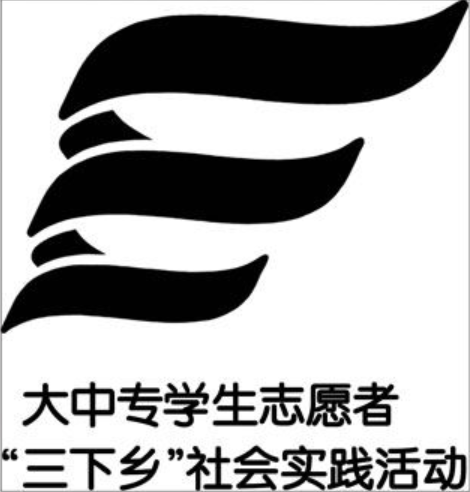
\includegraphics[width=2cm]{xiaxiang.png}
\end{minipage}
\end{figure*}
\end{spacing}

\end{document}